%\documentclass{article}
%\usepackage{graphicx,subfigure}
%\begin{document}

\begin{figure}[!h]
  \centering
  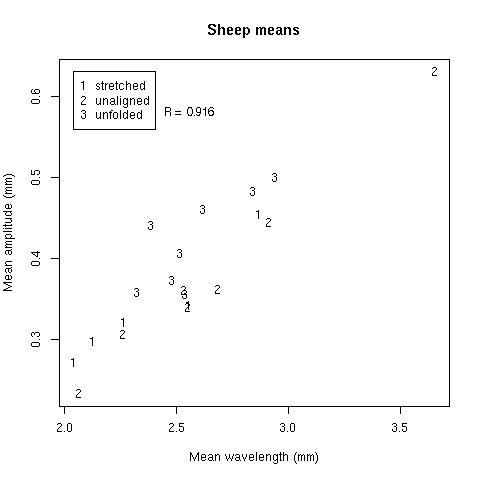
\includegraphics[width=1.0\textwidth]{figsfsheepmeans.png}
%   sheepmeanswa.png is original 
  \caption{Correlation between sheep means for Wavelength and Amplitude with CrimpType identified for each sheep. Means are averages over 15 fibres per sheep and 30 waves per fibre.}
  \label{fig:sfsheepmeans}
\end{figure}

%\end{document}

